\documentclass[12pt,a4paper]{report}
\usepackage[utf8]{inputenc}
\usepackage[T1]{fontenc}
\usepackage{graphicx}
\usepackage{geometry}
\usepackage{listings}
\usepackage{float}
\usepackage{hyperref}
\usepackage{xcolor}
\usepackage{amsmath}

\geometry{a4paper, margin=1in}

\definecolor{codegreen}{rgb}{0,0.6,0}
\definecolor{codegray}{rgb}{0.5,0.5,0.5}
\definecolor{codepurple}{rgb}{0.58,0,0.82}
\definecolor{backcolour}{rgb}{0.95,0.95,0.92}

\lstdefinestyle{mystyle}{
    backgroundcolor=\color{backcolour},
    commentstyle=\color{codegreen},
    keywordstyle=\color{magenta},
    numberstyle=\tiny\color{codegray},
    stringstyle=\color{codepurple},
    basicstyle=\ttfamily\footnotesize,
    breakatwhitespace=false,
    breaklines=true,
    captionpos=b,
    keepspaces=true,
    numbers=left,
    numbersep=5pt,
    showspaces=false,
    showstringspaces=false,
    showtabs=false,
    tabsize=2
}
\lstset{style=mystyle}

\begin{document}

\begin{titlepage}
\centering
\vspace*{1.5cm}

{\LARGE\textbf{CSE 4208: Computer Graphics Laboratory}\\}
\vspace{0.8cm}
{\Huge\textbf{SMART VILLAGE USING MODERN OPENGL}\\}
\vspace{1.5cm}

{\Large\textbf{By}\\}
\vspace{0.3cm}
{\Large SHrawosy Modak\\}
{\large Roll: 2007035\\}
\vspace{0.8cm}


\includegraphics[width=0.25\textwidth]{logo.png}\\
\vspace{0.8cm}

{\Large\textbf{Submitted To:}\\}
\vspace{0.4cm}
\begin{tabular}{p{0.42\textwidth} p{0.42\textwidth}}
\centering Dr. Sk. Md. Masudul Ahsan & \centering Md Tajmilur Rahman \\
\centering Professor & \centering Lecturer \\
\centering Dept. of CSE & \centering Dept. of CSE \\
\centering KUET & \centering KUET
\end{tabular}

\vfill

{\large Department of Computer Science and Engineering\\}
{\large Khulna University of Engineering \& Technology\\}
{\large Khulna 9203, Bangladesh\\}
{\large 8 April 2026\\}
\vspace{0.4cm}
{\small \copyright\ Dept. of CSE, KUET}

\end{titlepage}

\pagenumbering{roman}
\tableofcontents
\clearpage

\pagenumbering{arabic}

\chapter{Introduction}
This project presents the development of a "Smart Village," a comprehensive 3D environment designed and rendered using the OpenGL 3.3 API. Unlike static models, this scene is built procedurally to showcase the power of real-time computer graphics, featuring a detailed two-story school, a recreational park, and natural landscapes like rivers and forests. The implementation integrates core graphics concepts such as the Phong lighting model, texture mapping, and hierarchical transformations to create a visually rich and immersive experience. A key highlight of the project is the inclusion of mathematically derived objects, such as fractal-based trees and cubic B-spline surfaces for playground equipment. By providing an interactive interface with multiple camera viewports and dynamic lighting controls, the project offers a practical demonstration of a modern rendering pipeline. Ultimately, the "Smart Village" serves as a bridge between theoretical graphics algorithms and the technical execution of complex, interactive virtual worlds.

\section{Project Proposal}
\textbf{Proposal Name:} 3D Smart Village

This project proposal is to design an interactive 3D Smart Village scene in OpenGL where academic infrastructure, natural environment, and smart features are combined in one unified virtual world. In my implementation plan, the main structure is a detailed school area with surrounding houses, playground objects, river, trees, windmill, and road-side elements so that both static modeling and dynamic behavior can be demonstrated together.

The proposal focuses on using hierarchical modeling for complex objects, Phong-based lighting for day-night visual quality, and texture mapping for realistic surface appearance. It also includes mathematically generated curved geometry so that the scene is not limited to basic cubes only. For this reason, curved playground and environment objects are planned through Bezier curves, cubic B-spline, and ruled-surface based construction.

From an interaction perspective, the project is designed as a controllable simulation. The user can move with a flying camera, rotate the camera orientation, and switch between multiple shader modes. Dynamic state changes such as opening doors/windows, rotating windmill blades, and moving boat elements are included to make the world responsive instead of static. Lighting toggles (directional, point, spotlight, and ambient/diffuse/specular components) are also part of the proposal to evaluate different illumination setups in real time.

To improve observation and presentation quality, the proposal also includes multi-viewport rendering so the same scene can be analyzed from different camera configurations simultaneously. Overall, this proposal is aligned with the final smart village implementation goal: a technically rich OpenGL project that demonstrates modeling, texturing, lighting, animation, and user interaction within one coherent 3D environment.

\section{Background}
The evolution of real-time rendering has transformed how we visualize architectural and environmental data, shifting from simple wireframes to complex, hardware-accelerated simulations. This project is rooted in the study of the programmable graphics pipeline, where vertex and fragment shaders allow for precise per-pixel control over illumination and shading. The "Smart Village" theme was specifically chosen to provide a diverse testing ground for various geometric primitives, organic structures, and light-matter interactions within a single coordinate system. By leveraging the cross-platform capabilities of GLFW and GLAD, the project explores how low-level GPU programming can simulate realistic scenes and varied material properties. Understanding these fundamental building blocks is essential for developing high-performance applications in fields like urban planning, virtual reality, and gaming. It emphasizes the transition from basic rasterization to advanced shading techniques, such as the comparison between Gouraud and Phong reflection models.

\section{Objectives}
The project's major purpose is given below:
\begin{itemize}
    \item To build an interactive 3D Smart Village environment with a detailed school complex using OpenGL.
    \item To implement a multi-source lighting system including directional, point, and spotlights.
    \item To design and integrate complex curvy and organic objects such as fractal trees, B-spline slider, curved bench, cones, and cylinders.
    \item To enable dynamic user interaction through multi-view camera modes and interactive object states like opening doors and windows, rotating windmills, and moving clouds.
    \item To implement Bezier surface and ruled-surface modeling for curved objects.
\end{itemize}

\chapter{Project Implementation}
The project utilizes a custom rendering pipeline where every physical entity is either mathematically generated or parsed from external coordinate data. Figure 2.1 displays the structural layout of the entire scene from a global perspective.

\begin{figure}[h]
\centering
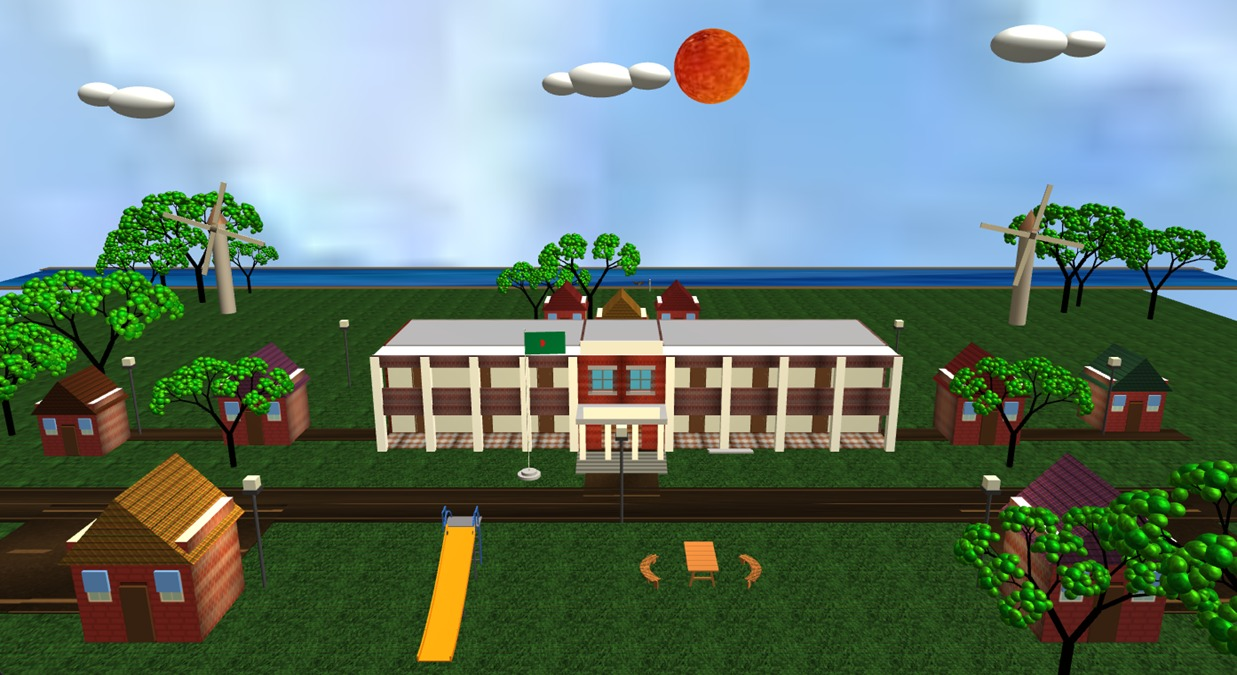
\includegraphics[width=0.8\textwidth]{full.jpeg}
\caption{3D Complete View of the Smart Village}
\label{fig:birdseye}
\end{figure}

\section{Physical Objects}
All objects in the simulation are modeled programmatically. By defining vertex attributes, including positions, normals for lighting, and UV coordinates for texturing, geometric precision is maintained across all scales.

\subsection{Cube}
The cube is the fundamental building block for the village's architecture, including the school walls, houses, and stairs. It consists of six faces formed by eight vertices. Each face is rendered using two triangles, ensuring compatibility with the OpenGL triangle primitive assembly.

Below are some codes responsible for cube.
\begin{lstlisting}[language=C++]
void drawCube(Shader& shader, glm::vec3 pos, glm::vec3 scale, glm::vec3 color, float shine, bool emissive) {
    glm::mat4 model = glm::translate(glm::mat4(1.0f), pos);
    model = glm::scale(model, scale);
    drawObject(shader, cubeVAO, 36, model, color, shine, emissive);
}
void drawObject(Shader& shader, unsigned int VAO, int vertexCount, glm::mat4 model, glm::vec3 color, float shine, bool emissive) {
    shader.setMat4("model", model);
    shader.setVec3("objectColor", color);
    shader.setFloat("shininess", shine);
    shader.setBool("isEmissive", emissive);
    if (emissive) {
        shader.setVec3("emissiveColor", color);
    }
    glBindVertexArray(VAO);
    glDrawArrays(GL_TRIANGLES, 0, vertexCount);
    if (emissive) {
        shader.setBool("isEmissive", false);
    }
}
\end{lstlisting}

\begin{figure}[h]
\centering
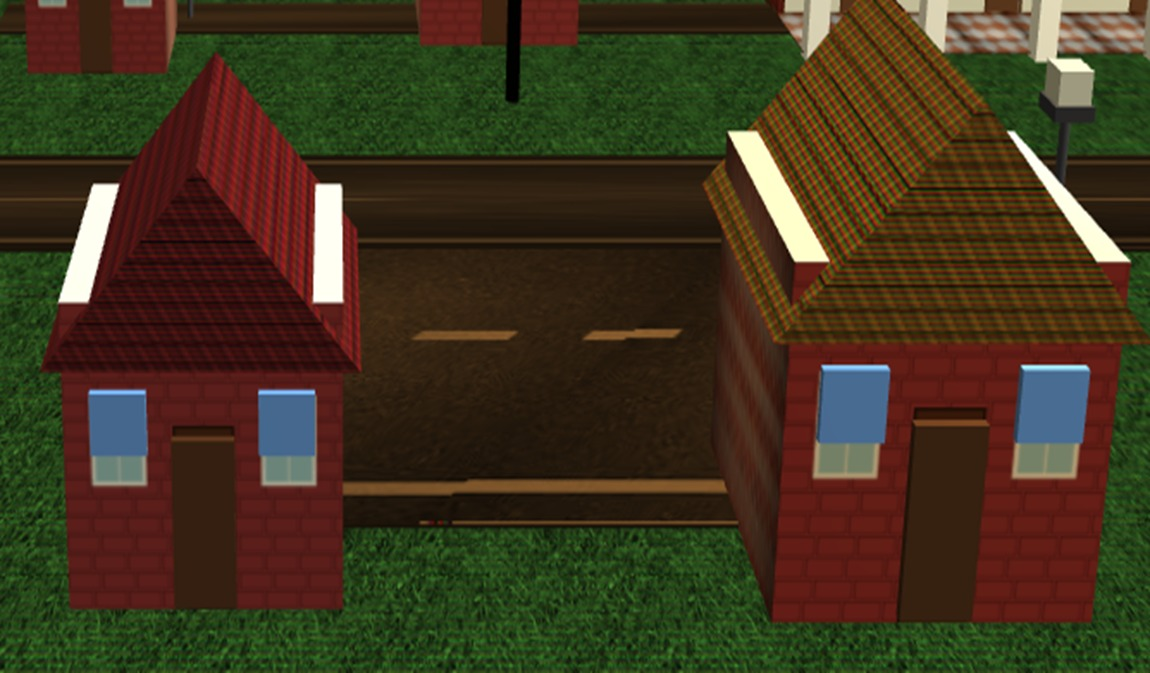
\includegraphics[width=0.6\textwidth]{house.jpeg}
\caption{House made with cube}
\end{figure}

\begin{figure}[h]
\centering
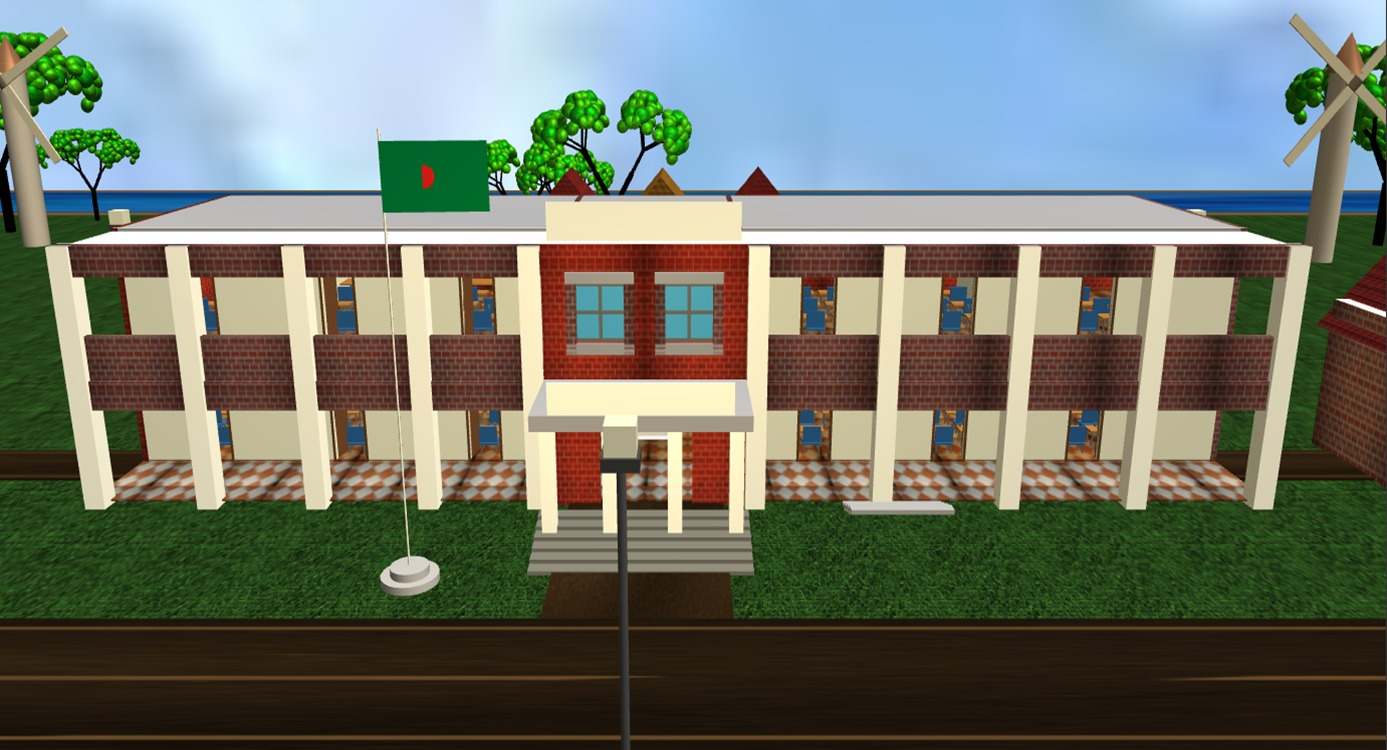
\includegraphics[width=0.6\textwidth]{school.jpeg}
\caption{School made with cube}
\end{figure}

\begin{figure}[h]
\centering
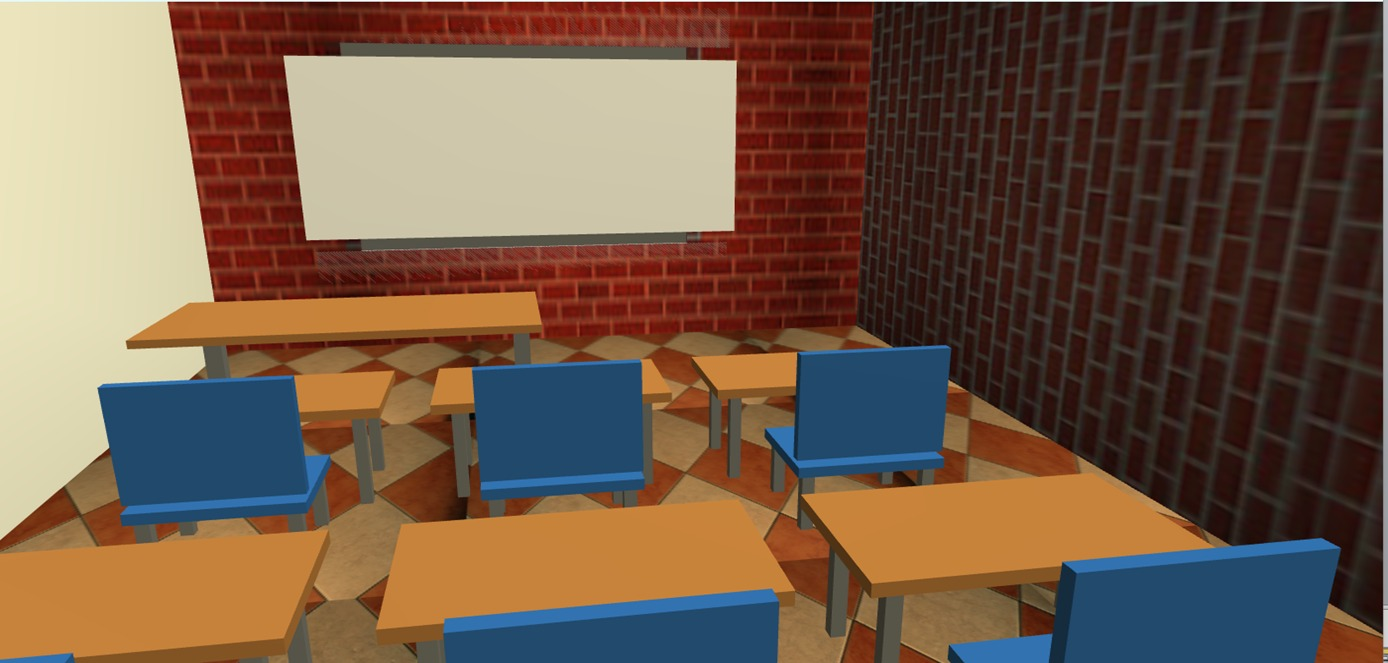
\includegraphics[width=0.6\textwidth]{classroom.jpeg}
\caption{Classroom made with cube}
\end{figure}

\subsection{Cylinder and Cone}
A cylinder has traditionally been a three-dimensional solid, one of the most basic of curvilinear geometric shapes. In this project, I used it while creating complex objects. It is used as the body of the windmill. Cylinders were modeled using circular bases and a curved surface connecting the two. Vertices are generated for the top and bottom circles by iterating over angles in a loop (using trigonometric functions for x and z coordinates). By setting one of the radii to zero, the same algorithm generates cones, which are used for decorative elements and lamp components. Vertices are calculated using trigonometric iterations:

\begin{center}
$x = r \cdot \cos(\theta)$

$z = r \cdot \sin(\theta)$
\end{center}

Below code show how cylinder and cone were generated in the project. Figure 2.5 shows the object generated with cone and cylinder.
\begin{lstlisting}[language=C++]
void drawCone(Shader& shader, glm::vec3 pos, glm::vec3 scale, glm::vec3 color, float shine, bool emissive) {
    glm::mat4 model = glm::translate(glm::mat4(1.0f), pos);
    model = glm::scale(model, scale);
    drawObject(shader, coneVAO, coneVertexCount, model, color, shine, emissive);
}

void drawCylinder(Shader& shader, glm::vec3 pos, glm::vec3 scale, glm::vec3 color, float shine, bool emissive) {
    glm::mat4 model = glm::translate(glm::mat4(1.0f), pos);
    model = glm::scale(model, scale);
    drawObject(shader, cylinderVAO, cylinderVertexCount, model, color, shine, emissive);
}
\end{lstlisting}

\begin{figure}[h]
\centering
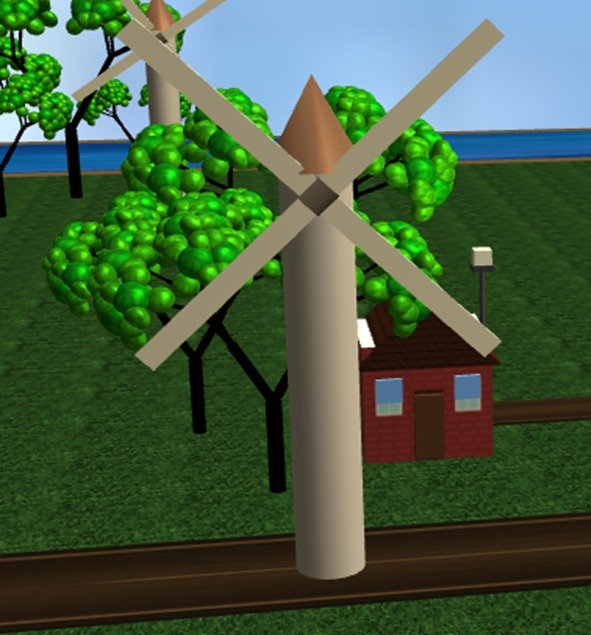
\includegraphics[width=0.6\textwidth]{windmill.jpeg}
\caption{Windmill made with Cylinder and Cone}
\end{figure}

\subsection{Fractal}
Fractal geometry is used in this project to generate procedural trees using recursive branching. The implementation uses a function \texttt{drawFractalBranch(...)} that draws one branch segment as a cylinder, then spawns two child branches until recursion depth becomes zero. The tree body uses \texttt{texTreeBody}, and leaf clusters at terminal depth use \texttt{texLeaf}.

For each recursion level, branch dimensions are reduced as:
\[
L_{k+1} = 0.75L_k, \qquad r_{k+1} = 0.65r_k
\]

If the starting depth is $d$, the total number of branch calls follows:
\[
N(d) = 2^{d+1} - 1
\]
because each branch generates two children (binary recursion).

In the scene, the tree is invoked with:
\begin{lstlisting}[language=C++]
drawFractalBranch(shader, baseModel, 2.5f * s, 0.4f * s, 5);
\end{lstlisting}

Below is the exact recursive branch generation logic from the project:
\begin{lstlisting}[language=C++]
void drawFractalBranch(Shader& shader, glm::mat4 model, float length, float radius, int depth) {
    glBindTexture(GL_TEXTURE_2D, texTreeBody);

    glm::mat4 branchModel = glm::translate(model, glm::vec3(0.0f, length / 2.0f, 0.0f));
    branchModel = glm::scale(branchModel, glm::vec3(radius, length, radius));
    drawCylinderModel(shader, branchModel, glm::vec3(0.02f, 0.02f, 0.02f), 8.0f, false);

    if (depth == 0) {
        glBindTexture(GL_TEXTURE_2D, texLeaf);
        glm::vec3 centerCol(0.15f, 0.85f, 0.25f);
        glm::mat4 centerLeaf = glm::translate(model, glm::vec3(0.0f, length * 1.1f, 0.0f));
        centerLeaf = glm::scale(centerLeaf, glm::vec3(radius * 18.0f, radius * 14.0f, radius * 18.0f));
        drawSphereModel(shader, centerLeaf, centerCol, 8.0f, false);

        for (int x = -1; x <= 1; x += 2) {
            for (int z = -1; z <= 1; z += 2) {
                glm::mat4 leafModel = glm::translate(model, glm::vec3(x * radius * 9.0f, length * 0.85f, z * radius * 9.0f));
                leafModel = glm::scale(leafModel, glm::vec3(radius * 14.0f, radius * 11.0f, radius * 14.0f));
                glm::vec3 outerCol = glm::vec3(0.35f + abs(x) * 0.15f, 0.95f, 0.15f + abs(z) * 0.1f);
                drawSphereModel(shader, leafModel, outerCol, 8.0f, false);
            }
        }
        return;
    }

    glm::mat4 endModel = glm::translate(model, glm::vec3(0.0f, length, 0.0f));
    float newLength = length * 0.75f;
    float newRadius = radius * 0.65f;

    glm::mat4 m1 = glm::rotate(endModel, glm::radians(30.0f), glm::vec3(0.0f, 0.0f, 1.0f));
    m1 = glm::rotate(m1, glm::radians(90.0f), glm::vec3(0.0f, 1.0f, 0.0f));
    drawFractalBranch(shader, m1, newLength, newRadius, depth - 1);

    glm::mat4 m2 = glm::rotate(endModel, glm::radians(-30.0f), glm::vec3(0.0f, 0.0f, 1.0f));
    m2 = glm::rotate(m2, glm::radians(90.0f), glm::vec3(0.0f, 1.0f, 0.0f));
    drawFractalBranch(shader, m2, newLength, newRadius, depth - 1);
}
\end{lstlisting}

\begin{figure}[h]
\centering
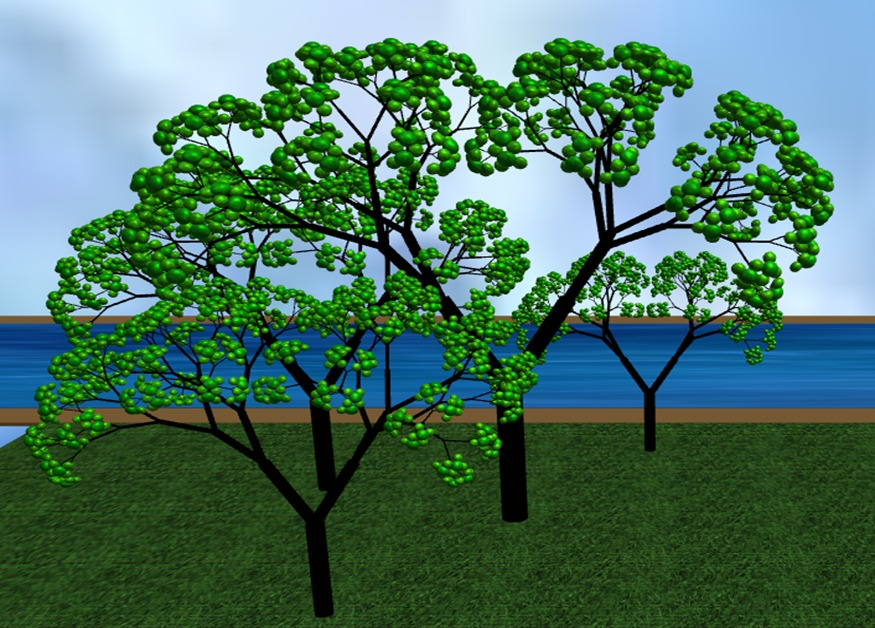
\includegraphics[width=0.6\textwidth]{tree.jpeg}
\caption{Fractal Tree used in the project}
\end{figure}

\section{Lighting Controls}
Lighting in this project is controlled through runtime toggles and implemented with a Phong-based model in the fragment shader. Three light categories are used: directional light , multiple point lights (street lamps), and one spotlight.

The following toggles are implemented in input handling:
\begin{table}[h]
\centering
\caption{Lighting toggle keys used in the project}
\begin{tabular}{|l|l|}
\hline
\textbf{Key} & \textbf{Activity} \\
\hline
1 & Toggle directional light (ON/OFF) \\
2 & Toggle all point lights (ON/OFF) \\
3 & Toggle spotlight (ON/OFF) \\
5 & Toggle ambient component \\
6 & Toggle diffuse component \\
7 & Toggle specular component \\
\hline
\end{tabular}
\end{table}

The final lighting sum is:
\[
I_{\text{final}} = I_{\text{dir}} + \sum_{i=1}^{N} I_{\text{point},i} + I_{\text{spot}}
\]
where each term contributes ambient, diffuse, and specular parts depending on toggle states.

\subsection{Point Light}
A point light emits equally in all directions from lamp positions. In this project, multiple street lamps are stored in \texttt{streetLampPositions} and sent to shader arrays .

\begin{figure}[H]
\centering
\includegraphics[width=0.45\textwidth]{point.jpeg}
\caption{Point light activated in the scene}
\end{figure}

Distance attenuation is computed by:
\[
\text{attenuation} = \frac{1}{k_c + k_l d + k_q d^2}
\]
with project constants:
\[
k_c = 1.0, \quad k_l = 0.09, \quad k_q = 0.032
\]



\begin{lstlisting}[language=GLSL]
vec3 CalcPointLight(int index, vec3 normal, vec3 fragPos, vec3 viewDir)
{
    vec3 lightPos = pointLightPos[index];
    vec3 lightColor = pointLightColor[index];
    vec3 lightDir = normalize(lightPos - fragPos);

    float distance = length(lightPos - fragPos);
    float attenuation = 1.0 / (pointLightConstant + pointLightLinear * distance +
                               pointLightQuadratic * (distance * distance));

    vec3 ambient = enableAmbient ? 0.1 * lightColor * attenuation : vec3(0.0);
    vec3 diffuse = vec3(0.0);
    if (enableDiffuse) {
        float diff = max(dot(normal, lightDir), 0.0);
        diffuse = diff * lightColor * attenuation;
    }

    vec3 specular = vec3(0.0);
    if (enableSpecular) {
        vec3 reflectDir = reflect(-lightDir, normal);
        float spec = pow(max(dot(viewDir, reflectDir), 0.0), shininess);
        specular = spec * lightColor * 0.5 * attenuation;
    }

    return (ambient + diffuse + specular);
}
\end{lstlisting}

\subsection{Spotlight}
The spotlight is implemented as a focused cone light with soft edge falloff. In this project, one spotlight source is configured with:
\[
\text{position}=(0.0, 4.8, 12.0), \quad
\text{direction}=\text{normalize}((0.0,4.0,0.0)-(0.0,4.8,12.0))
\]
\[
\text{cutOff}=\cos(10^\circ), \quad
\text{outerCutOff}=\cos(15^\circ), \quad
\text{intensity}=4.0
\]

\begin{figure}[H]
\centering
\includegraphics[width=0.42\textwidth,height=0.24\textheight,keepaspectratio]{spot.jpeg}
\caption{Spotlight on road lamppost}
\end{figure}

Cone intensity is:
\[
\theta = \hat{L} \cdot (-\hat{D}), \quad
\epsilon = \text{cutOff} - \text{outerCutOff}
\]
\[
I_{\text{cone}} = \text{clamp}\left(\frac{\theta-\text{outerCutOff}}{\epsilon}, 0, 1\right)
\]
and final spotlight factor is multiplied by distance attenuation and \texttt{spotlightIntensity}.

\begin{table}[h]
\centering
\caption{Keyboard activity triggering spotlight control}
\begin{tabular}{|l|l|}
\hline
\textbf{Key} & \textbf{Activity} \\
\hline
Key 3 & Toggling spotlight ON/OFF \\
\hline
\end{tabular}
\end{table}

\begin{lstlisting}[language=GLSL]
vec3 CalcSpotlight(vec3 normal, vec3 fragPos, vec3 viewDir)
{
    vec3 lightDir = normalize(spotlightPos - fragPos);
    float theta = dot(lightDir, normalize(-spotlightDir));
    float epsilon = spotlightCutOff - spotlightOuterCutOff;
    float intensity = clamp((theta - spotlightOuterCutOff) / epsilon, 0.0, 1.0);

    if (theta < spotlightOuterCutOff) return vec3(0.0);

    float distance = length(spotlightPos - fragPos);
    float attenuation = 1.0 / (1.0 + 0.09 * distance + 0.032 * (distance * distance));
    float finalIntensity = attenuation * intensity * spotlightIntensity;

    vec3 ambient = enableAmbient ? 0.1 * spotlightColor * finalIntensity : vec3(0.0);
    float diff = max(dot(normal, lightDir), 0.0);
    vec3 diffuse = enableDiffuse ? diff * spotlightColor * finalIntensity : vec3(0.0);

    vec3 specular = vec3(0.0);
    if (enableSpecular) {
        vec3 reflectDir = reflect(-lightDir, normal);
        float spec = pow(max(dot(viewDir, reflectDir), 0.0), shininess);
        specular = spec * spotlightColor * finalIntensity;
    }

    return (ambient + diffuse + specular);
}
\end{lstlisting}

\subsection{Directional Light}
Directional light simulates sunlight in day mode and moon-like lighting in night mode. Day and night parameters are updated from CPU-side uniforms.


For directional light:
\[
I_{\text{dir}} = I_a + I_d + I_s
\]
\[
I_d = \max(\hat{N}\cdot\hat{L}, 0), \qquad
I_s = \max(\hat{V}\cdot\hat{R}, 0)^{\text{shininess}}
\]
where $\hat{R}=\text{reflect}(-\hat{L},\hat{N})$.

\begin{table}[h]
\centering
\caption{Keyboard activity triggering directional light control}
\begin{tabular}{|l|l|}
\hline
\textbf{Key} & \textbf{Activity} \\
\hline
Key 1 & Toggling directional light \\
\hline
\end{tabular}
\end{table}

\begin{lstlisting}[language=C++]
// From setLightingUniforms(...)
if (isNightMode) {
    shader.setVec3("sunDirection", glm::vec3(0.2f, -0.8f, 0.3f));
    shader.setVec3("sunAmbient",  glm::vec3(0.05f, 0.05f, 0.1f));
    shader.setVec3("sunDiffuse",  glm::vec3(0.1f, 0.1f, 0.2f));
    shader.setVec3("sunSpecular", glm::vec3(0.15f, 0.15f, 0.25f));
} else {
    shader.setVec3("sunDirection", glm::vec3(-0.4f, -0.8f, -0.3f));
    shader.setVec3("sunAmbient",  glm::vec3(0.35f, 0.35f, 0.32f));
    shader.setVec3("sunDiffuse",  glm::vec3(0.95f, 0.95f, 0.9f));
    shader.setVec3("sunSpecular", glm::vec3(1.0f, 1.0f, 0.95f));
}
\end{lstlisting}

\begin{lstlisting}[language=GLSL]
vec3 CalcDirectionalLight(vec3 normal, vec3 viewDir)
{
    vec3 lightDir = normalize(-sunDirection);
    vec3 ambient = enableAmbient ? sunAmbient : vec3(0.0);

    vec3 diffuse = vec3(0.0);
    if (enableDiffuse) {
        float diff = max(dot(normal, lightDir), 0.0);
        diffuse = diff * sunDiffuse;
    }

    vec3 specular = vec3(0.0);
    if (enableSpecular) {
        vec3 reflectDir = reflect(-lightDir, normal);
        float spec = pow(max(dot(viewDir, reflectDir), 0.0), shininess);
        specular = spec * sunSpecular;
    }

    return ambient + diffuse + specular;
}
\end{lstlisting}

\section{Texturing}
Textures in this project are assigned by object type. The sphere is used for the sun and football, the cylinder is used for the tree body and windmill body, and the cone is used for the windmill top. Cube textures are used for the buildings and other box-shaped parts.

\subsection{On Cube}
Cube faces use separate texture mapping for walls, roofs, doors, windows, and other box-like parts of the scene.

\subsection{On Sphere}
Sphere mapping is used for the sun and football, where UV coordinates are generated from the spherical surface.

\subsection{On Cylinder}
Cylinders are textured on the tree trunk, windmill body, and other round parts by wrapping the texture around the curved surface.

\subsection{On Cone}
Cones are textured on the windmill top and similar pointed parts.

\begin{figure}[h]
\centering
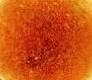
\includegraphics[width=0.46\textwidth,height=0.22\textheight,keepaspectratio]{sun.jpeg}
\hfill

\caption{Texture of sun used in the project}
\end{figure}

\section{Blending Multiple Shader}
A methodology applied in this project, where texture color is combined with lighting result to get the final pixel color. Three rendering modes are implemented in the project: Mode 1 for simple texture rendering, Mode 2 for blended Gouraud shading, and Mode 3 for blended Phong shading.

\begin{table}[h]
\centering
\caption{Keyboard activity triggering blending controls}
\begin{tabular}{|l|l|}
\hline
\textbf{Mode} & \textbf{Activity} \\
\hline
Mode 1 (Key N) & Simple texture with Phong lighting \\
Mode 2 (Key M) & Blended Gouraud shading \\
Mode 3 (Key O) & Blended Phong shading \\
\hline
\end{tabular}
\end{table}

\begin{figure}[h]
\centering
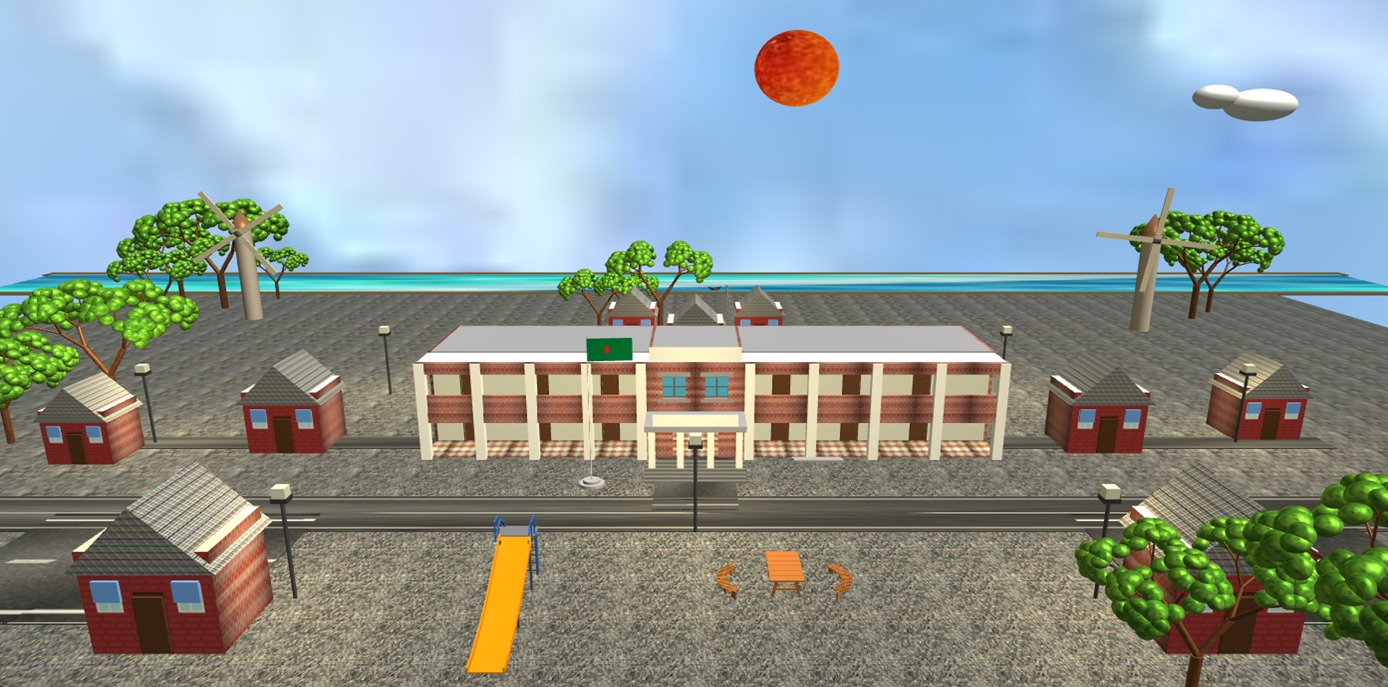
\includegraphics[width=0.46\textwidth,height=0.25\textheight,keepaspectratio]{texture1.jpeg}
\hfill
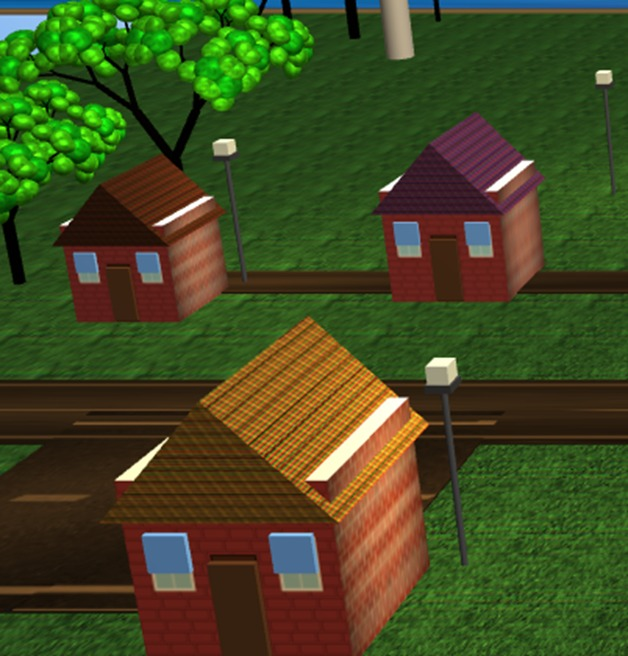
\includegraphics[width=0.46\textwidth,height=0.25\textheight,keepaspectratio]{texture2.jpeg}
\caption{Simple texture and Blended Phong rendering results}
\end{figure}

\section{Curvy Object Integration}
Curvy objects in this project are generated with three curve families: Bezier curve, cubic B-spline, and ruled surface. The boat uses Bezier-based hull shaping, the slide uses a clamped cubic B-spline with ruled side walls and Bezier handrails, and the picnic bench uses cubic B-spline curve segments with ruled surface connections.

\begin{table}[H]
\centering
\caption{Curve type used for each curvy object}
\begin{tabular}{|l|l|l|}
\hline
\textbf{Object} & \textbf{Curve type} & \textbf{Use in the project} \\
\hline
Boat & Bezier curve & Smooth hull profile and body shaping \\
Bench & Cubic B-spline & Curved seating path and bench form \\
Slider & B-spline + ruled surface + Bezier & Slide surface, side walls, and handrails \\
\hline
\end{tabular}
\end{table}

\subsection{Boat}
The boat is built with Bezier-based hull profiles. The hull is generated from smooth profile control points, and the surface is closed with triangular and quad patches.

\begin{figure}[H]
\centering
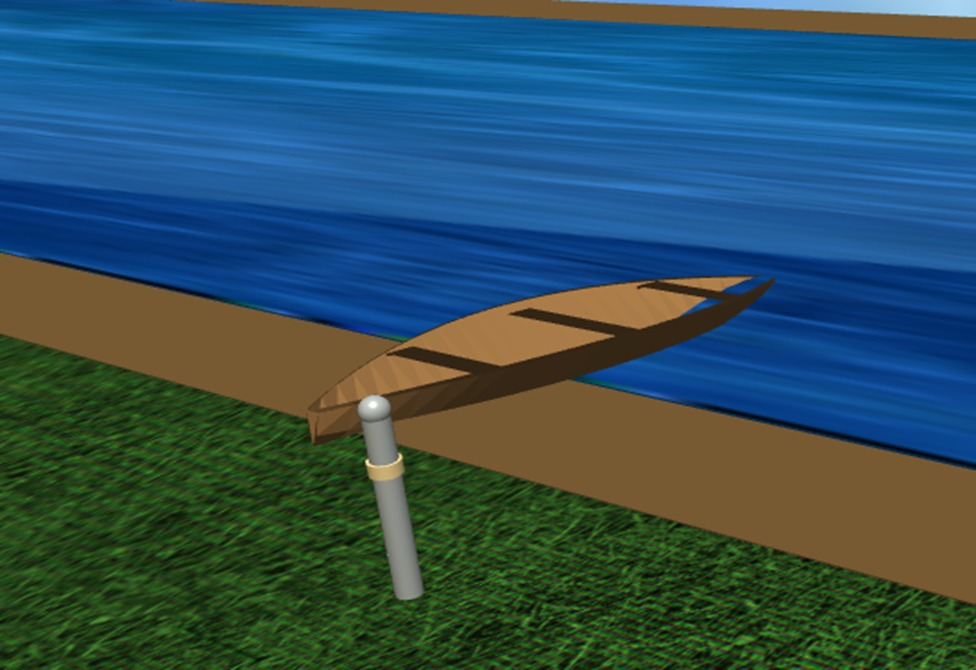
\includegraphics[width=0.6\textwidth,height=0.26\textheight,keepaspectratio]{boat.jpeg}
\caption{Boat generated using Bezier curve}
\end{figure}

\subsection{Bench}
The picnic bench uses cubic B-spline segments for the curved seating arrangement, while ruled surface connections are used for the slats and supports.

\begin{figure}[H]
\centering
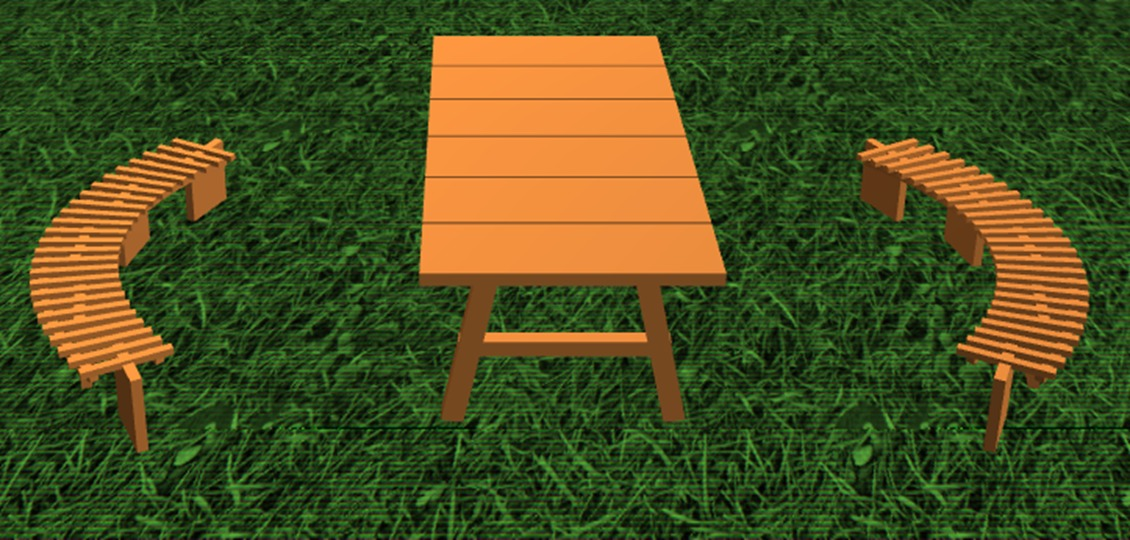
\includegraphics[width=0.6\textwidth,height=0.26\textheight,keepaspectratio]{bench.jpeg}
\caption{Curved bench generated using B-spline curve}
\end{figure}

\subsection{Slider}
The playground slider is generated using a clamped cubic B-spline for the chute, ruled surfaces for the side walls, and cubic Bezier curves for the handrails.

\begin{figure}[H]
\centering
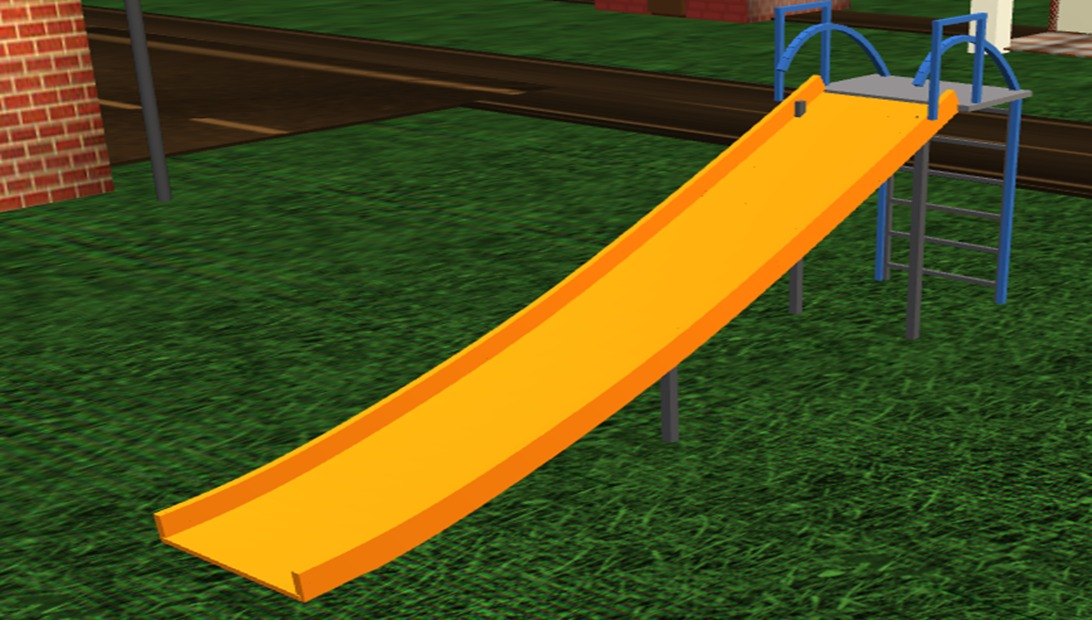
\includegraphics[width=0.6\textwidth,height=0.26\textheight,keepaspectratio]{slider.jpeg}
\caption{Slider generated using B-spline, ruled surface, and Bezier curve}
\end{figure}

\section{Dynamic Interactions (Keyboard Functionalities)}
To make the scene dynamic and interactive, keyboard controls were implemented for camera movement, camera modes, lighting toggles, shader mode changes, and object state changes (doors and windows). These functionalities are handled through real-time input processing.


\begin{table}[H]
\centering
\caption{Keyboard activity triggering dynamic interaction}
\begin{tabular}{|l|l|}
\hline
\textbf{Key} & \textbf{Activity} \\
\hline
W, A, S, D & Move the camera forward, left, backward, right \\
E, R & Move camera up and down \\
X, Y, Z & Camera pitch, yaw, and roll control \\
F, HOME & Orbit mode toggle and camera reset \\
P, U & Open/close doors and windows \\
V & Toggle four-viewport split screen \\
N, M, O & Mode 1, Mode 2, Mode 3 shader mode switch \\
\hline
\end{tabular}
\end{table}

\begin{figure}[H]
\centering
\includegraphics[width=0.82\textwidth,height=0.36\textheight,keepaspectratio]{dynamic_demo.jpg}
\caption{Dynamic Interactions in the Scene}
\end{figure}


\clearpage
\chapter{Viewport System}
The project supports both single-view rendering and four-viewport split rendering. By pressing \texttt{V}, the renderer switches between normal full-screen view and a 2x2 viewport layout. The four-way layout is used for simultaneous observation from different camera setups, including top/bird view and perspective side views.

\begin{table}[H]
\centering
\caption{Viewport control in the project}
\begin{tabular}{|l|l|}
\hline
\textbf{Key} & \textbf{Activity} \\
\hline
V & Toggle 4-viewport split screen ON/OFF \\
B & Bird's-eye camera preset \\
\hline
\end{tabular}
\end{table}

\begin{figure}[H]
\centering
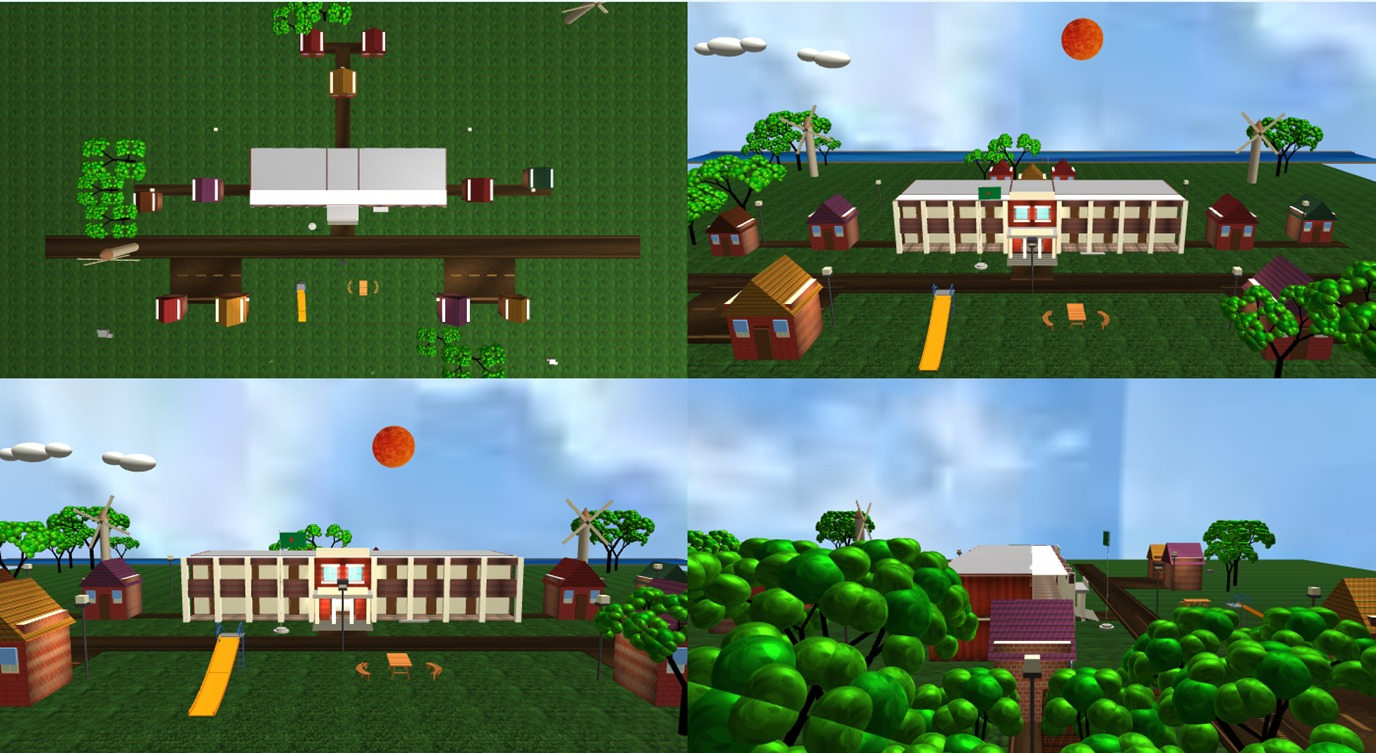
\includegraphics[width=0.82\textwidth,height=0.36\textheight,keepaspectratio]{viewport.jpeg}
\caption{Viewport rendering mode in the project}
\end{figure}


\chapter{Conclusions}
This project effectively demonstrates the capability of OpenGL to create a dynamic and interactive 3D simulation of a city. Through the use of texture mapping, lighting, geometric modeling, and interactive features, the project delivers a visually engaging and realistic urban environment. Static and dynamic elements, such as curvy objects and user-controlled vehicles, enhance the scene's depth. Future improvements could involve optimizing performance, adding more advanced features, and incorporating higher levels of detail to make the simulation more immersive and versatile.

\section{Conclusion and challenges faced}
The development of project presented several challenges that required iterative refinement and problem-solving. Performance optimization was a key hurdle, as maintaining frame rates and ensuring smooth rendering in a complex scene with multiple dynamic objects proved difficult. Lighting, such as balancing the intensity and positioning of point lights and spotlights, was necessary to achieve realism without overexposure. Implementing Bezier curves and fractals required a deep understanding of mathematics, while texture mapping on irregular shapes like spheres and cones demanded meticulous alignment. Integrating external Blender models into the OpenGL environment without losing detail was another significant challenge. Additionally, designing responsive keyboard inputs and maintaining the realism of dynamic interactions further tested the robustness of the implementation. Overcoming these provided invaluable insights and practical skills.

\begin{thebibliography}{9}
\bibitem{demko}
Demko, Stephen, Laurie Hodges, and Bruce Naylor. "Construction of fractal objects with iterated function systems." Proceedings of the 12th annual conference on Computer graphics and interactive techniques. 1985.

\bibitem{farin}
Farin, Gerald. "Class a Bezier curves." Computer aided geometric design 23.7 (2006): 573-581.

\bibitem{shreiner}
Shreiner, Dave, et al. "OpenGL Programming Guide: The Official Guide to Learning OpenGL." Addison-Wesley Professional, 2013.
\end{thebibliography}

\end{document}
